
\subsection{Reduced model for the $(2,0)$ fuzzy Dirac operator}
The purpose of this section is to apply the tools of random matrix theory to the study of the simplest non-trivial model, namely the type $(2,0)$ Dirac operator. The general idea is to identify degrees of freedom that can be integrated out, and to write a simpler model in terms of the remaining ones.\newline
First a more convenient notation for the model is introduced, then the classical solutions are found and finally the simplified model is obtained by considering small perturbations of these.\newline
This project is work in progress with Professor Sven Gnutzmann.

\subsubsection{Notation}
Throughout this section a more convenient notation is used in order to properly identify the relevant degrees of freedom.\newline
Recall that a type $(2,0)$ Dirac operator is written as:
\begin{equation}
D = \gamma_1 \otimes \{H_1, \cdot \} + \gamma_2 \otimes \{H_2, \cdot \}
\end{equation}
for Hermitian matrices $H_1$ and $H_2$. Define $\gamma_{\pm} := \frac{1}{2}(\gamma_1 \mp i \gamma_2)$ and $W := H_1 + i H_2$ and rewrite $D$ in these terms:
\begin{equation}
D = \gamma_+ \otimes \{ W, \cdot \} + \gamma_- \otimes \{ W^\dagger, \cdot \}.
\end{equation}
The quadratic and quartic terms in the action read:
\begin{align}
\Tr D^2 &= 4 (n \Tr W W^{\dagger} + \Tr W \Tr W^{\dagger}) \\ 
\Tr D^4 &= 4 \big[ n \Tr(W W^\dagger)^2 + \Tr W^2 \Tr W^{\dagger 2} + 2 (\Tr W W^\dagger)^2 \notag \\ 
&+ 2 \Tr W^2 W^\dagger \Tr W^\dagger + 2 \Tr W^{\dagger 2} W \Tr W \big].
\end{align}


\subsubsection{Stationary manifold}
Stationary points are solutions to the equations of motion:
\begin{equation}
\delta S = S[W + \delta W] - S[W] = 0 \quad  \forall \ \delta W \ll 1.
\end{equation}
To first order in $\delta W$ and $\delta W^\dagger$ the terms $\Tr D^2$ and $\Tr D^4$ give:
\begin{align}
\delta \Tr D^2 &= 4 \Tr \Big\{ [1+ \dagger] [ n W + (\Tr W) I ] \delta W^\dagger \Big\} \\
\notag \\
\delta \Tr D^4 &= 4 \Tr \Big\{ [1+ \dagger] [2n W W^\dagger W  + (2 \Tr W^2) W^\dagger  + (4 \Tr W W^\dagger) W + \notag \\
&\phantom{aaaaaaa} (2 \Tr W^2 W^\dagger) I + (2 \Tr W^\dagger) W^2 + \notag \\ 
&\phantom{aaaaaaa}(2 \Tr W) ( W^\dagger W + W W^\dagger )] \delta W^\dagger \Big\}.
\end{align}
Solutions are found by putting the coefficient of $\delta W$ or $\delta W^\dagger$ to zero. They are of the form:
\begin{equation}
W = I \rho e^{i \theta}
\end{equation}
where
\begin{equation}
\rho^2 = 0 \quad \text{or} \quad \rho^2 = -\frac{g}{8}
\end{equation}
and $\theta$ is unconstrained.
\subsubsection{Small oscillations and quadratic action}
Write $W = \eit(\rho + \epsilon V)$ for small $\epsilon$ and traceless $V$. Order by order in $\epsilon$, the contributions to the action are:
\begin{align}
\Tr D^2 \notag \\
O(1)&: \quad 8n^2 \rho^2 \\
O(\epsilon)&: \quad 8n \rho ( \Tr V^\dagger + \Tr V) \\
O(\epsilon^2)&: \quad 4 (n \Tr V V^\dagger + \Tr V \Tr V^\dagger) \\
\\ \notag
\Tr D^4 \notag \\
O(1)&: \quad 32n^2 \rho^4 \\
O(\epsilon)&: \quad 48 n \rho^3 (\Tr V^\dagger + \Tr V) \\
O(\epsilon^2)&: \quad 16 \rho^2(2n \Tr V V^\dagger + n \Tr V V \\
&\phantom{:\quad \ }+2 \Tr V \Tr V^\dagger + \Tr V \Tr V + \text{c.c.}) \notag 
\end{align}
Since $V$ is traceless, the action to second order in $\epsilon$ reads:
\begin{equation}\label{eq:quadr}
S = 8n^2(g \rho^2 + 4 \rho^4) + 2n \epsilon^2 \Tr(\vec{V}^T M \vec{V}) 
\end{equation}
with $\vec{V}^T = (V, V^\dagger)$ and:
\begin{equation}
M = \begin{bmatrix}
    8 \rho^2 & g + 16 \rho^2 \\
    g + 16 \rho^2 & 8 \rho^2 \\
\end{bmatrix}.
\end{equation}
At this point the idea would be to perform the gaussian integral in $V$ and remain with an effective theory in $\rho$. As it turns out, the contribution of $V$ cannot be integrated out due to the fact that $M$ has a zero eigenvalue on the stationary solutions. This signals the presence of modes that are not confined by a quadratic potential (\textit{massless zero modes}). The issue can be made explicit by decomposing $V = A + iB$ for Hermitian and traceless $A$ and $B$. In these variables the action (\ref{eq:quadr}) reads:
\begin{equation}
S = 8n^2(g \rho^2 + 4 \rho^4) + 4n \epsilon^2 \Big[ (g+24\rho^2) \Tr A^2 + (g+8\rho^2) \Tr B^2 \Big]
\end{equation}
where the coefficient of the $B$ part vanishes on the stationary solutions $\rho^2 = -g/8$. This suggests that one needs to go to higher orders in perturbation theory to find a confining potential for $B$. Numerical simulations confirm this picture (see Fig.(\ref{fig:ab})). 
\begin{figure}[hp]
\centering
\textbf{Norm of $A$ and $B$}
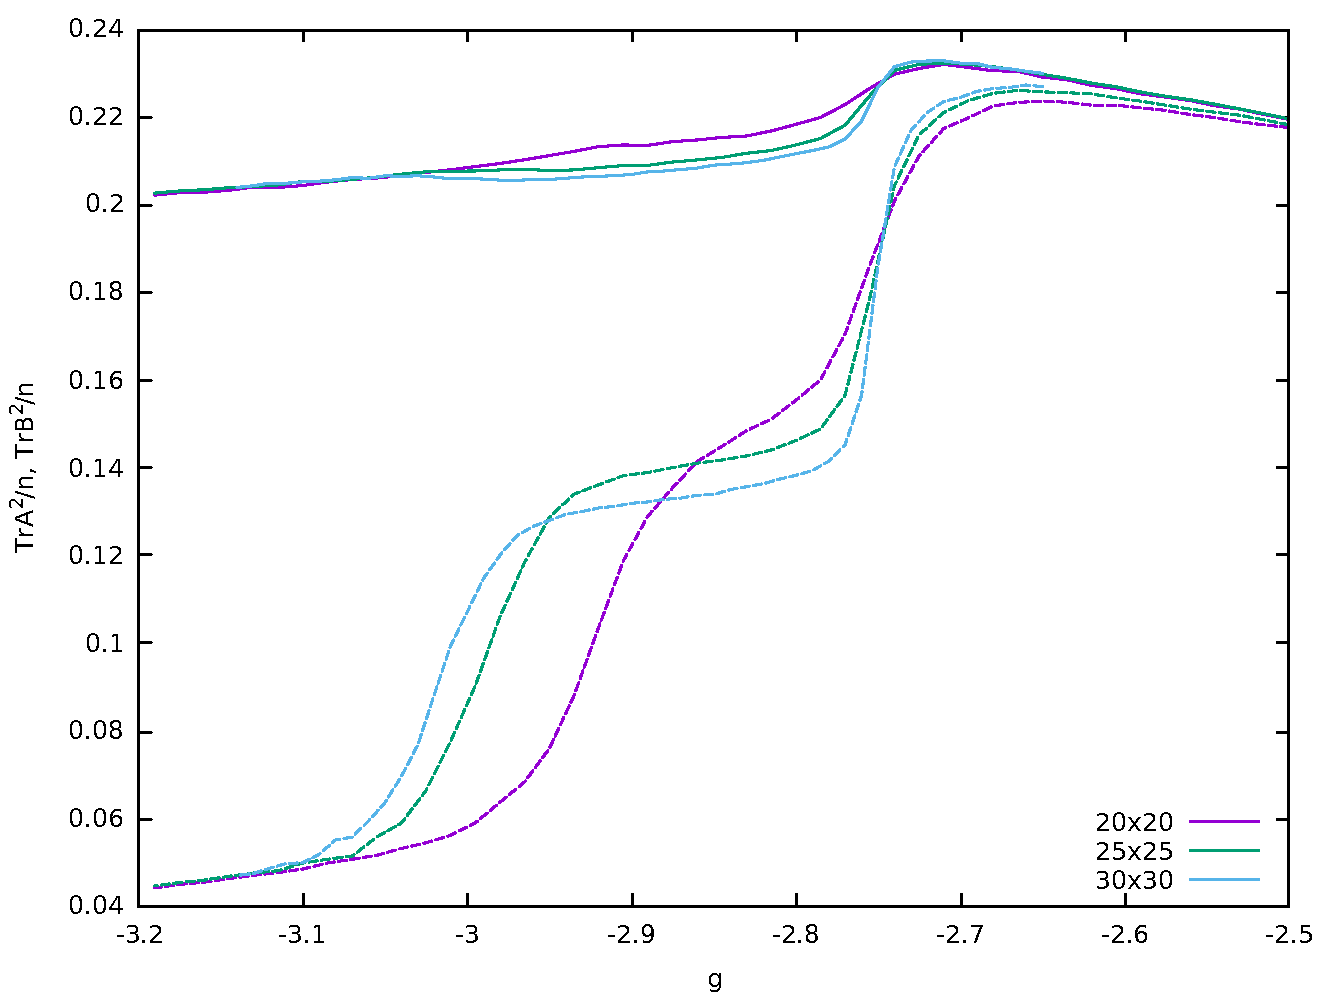
\includegraphics[width=1\linewidth]{fig/ab.pdf}
\caption{$\Tr A^2/n$ (dotted lines) and $\Tr B^2/n$ (solid lines) versus coupling constant $g$ for $n = 20 \ (\text{purple}), 25 \ (\text{green}), 30 \ (\text{blue})$ at the phase transition.}
\label{fig:ab}
\end{figure}